%\section{Different refract index}
From this section we begin to investigate optimal methods in the third propagating track: waveguide. The refractive index of the waveguide can also affect the coupling ability. In this section the effect of varying refractive index for coupling will be discussed. The experimental setup of the waveguide is substrate with index $n=1.544$ and guide with index $n=2.516$. For simplifying the simulation the substrate setup is kept and only the refractive indexes of the guide is varied from $1.6$ to $2.5$ in this section.\\

\begin{figure}[!ht]
\centering
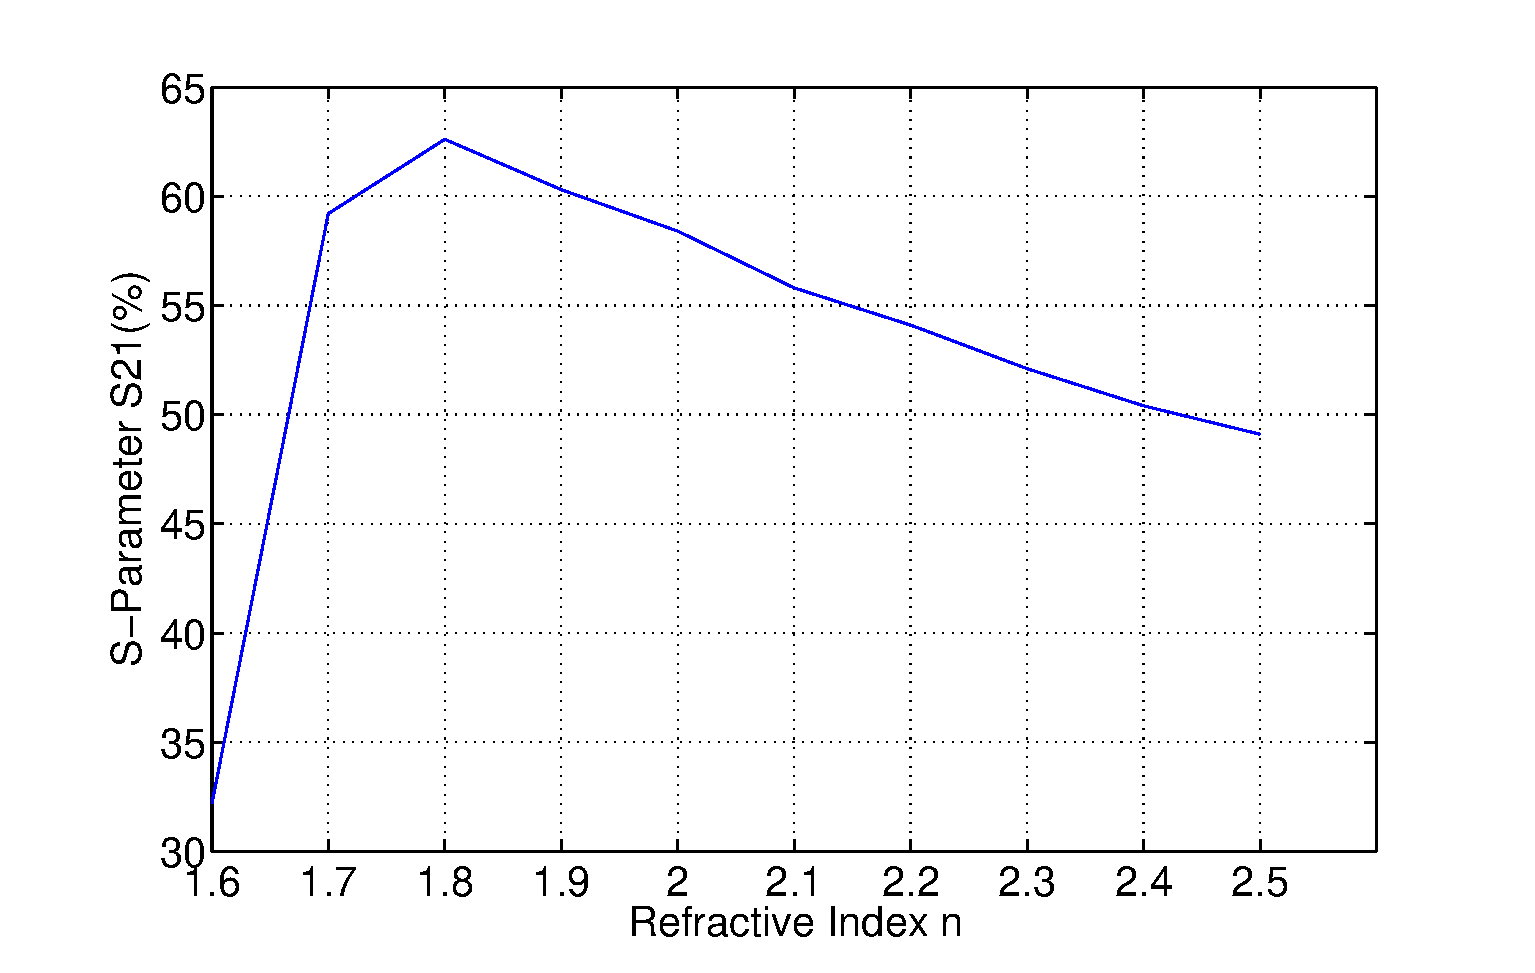
\includegraphics[width=0.6\textwidth]{bilder/s21_refractive_index}
\caption{Coupling efficiency between TLF and the rib waveguide at $f=282$THz due to refractive indices.}
\label{fig:refractive_index}
\end{figure}
Fig. \ref{fig:refractive_index} exhibits simulation results of this arrangement at working frequency of $282$ THz. It can be told from the figure that the coupling ability rises sharply from $n=1.6$ to $1.8$ and decline gently to $n=2.5$. It can also be derived that coupling efficiency will be decreased with the increasing of refractive indexes if $n>2.5$. Thus there is no need to do more simulations for other indexes of $n>2.5$. The highest value of the coupling efficiency among this index range is about $62.6\%$ when the guide is composed of material of $n=1.8$.\\

The reason for this behavior in the figure is complicated. First agenda is the numerical aperture (NA). In order to match the focal light from the TLF, the minimal NA should be larger than $0.798$. Using equation (\ref{eq:NA}) the NA for index $1.6$ is obtained by
\begin{equation*}
\sqrt{n_{1}^2-n_{2}^2}=\sqrt{1.6^2-1.544^2}=0.42.
\end{equation*}
This value is smaller than above request. Thus heavy power loss occurs at the end face of the waveguide. The value of NA is raised with the index increasing, $0.711$ for $n=1.7$ and $0.925$ for $n=1.8$.  When the index is still expanding other aspects become dominated. One aspect is the reflection at the end face. Fig. \ref{fig:s11_index} collects the relation between reflection and indices. After index of $1.7$ reflection is proportional to the value of the index. Combing other aspects of power loss the coupling efficiency falls after index of $1.9$.\\
  
\begin{figure}[!ht]
\centering
\includegraphics[width=0.6\textwidth]{bilder/s11_index}
\caption{Reflection due to refractive indices.}
\label{fig:s11_index}
\end{figure}

To conclusion the most efficient material of guide here is the one with index $n=1.8$.  Surely, it is not possible to find the material of any refractive index. If we want to improve the coupling ability by this means, the material with a refractive index close to $n=1.8$ can be optional.
